% uid: ""
% school: "lycee"
% level: "1ere"
% chapter: "Théorème de Thalès et sa réciproque"
% title: "Aires dans un trapèze"
% difficulty: "Difficile"
% tags: ["thales", "papillon", "aires", "trapeze"]
% provenance: "own"
% batch: "2026-11-22-revision-1ere-A"

% ---STATEMENT---
$ABCD$ est un trapèze de bases $[AB]$ et $[DC]$, avec $AB=a<DC=b$. Ses diagonales se coupent en $O$. On note $S_1$, $S_2$, $S_3$ et $S_4$ les aires des triangles $OAB$, $OCD$, $OAD$ et $OBC$.
% alt: Trapèze ABCD de bases AB et DC, diagonales sécantes en O, triangles OAB et OCD marqués
\begin{center}
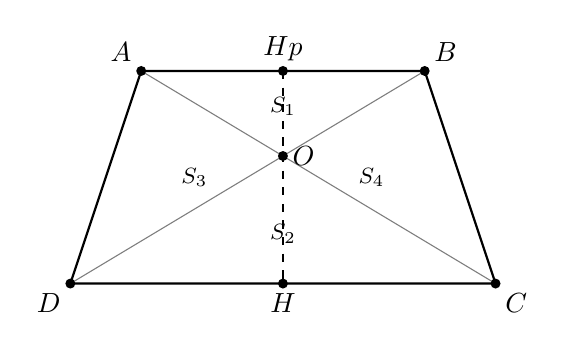
\begin{tikzpicture}[scale=0.9]
  \coordinate (D) at (0,0); \coordinate (C) at (6,0); \coordinate (A) at (1,3); \coordinate (B) at (5,3); \coordinate (O) at (3,1.8);
  \coordinate (H) at (3,0); \coordinate (Hp) at (3,3);
    \draw[thick] (A)--(B)--(C)--(D)--cycle; \draw[gray] (A)--(C); \draw[gray] (B)--(D); \draw[dashed] (Hp)--(H);
  \foreach \p/\pos in {A/above left,B/above right,C/below right,D/below left,O/right,H/below,Hp/above}{\fill (\p) circle (2pt) node[\pos]{$\p$};}
  \node at (3,2.5) {\footnotesize$S_1$}; \node at (3,0.7) {\footnotesize$S_2$}; \node at (1.75,1.5) {\footnotesize$S_3$}; \node at (4.25,1.5) {\footnotesize$S_4$};
\end{tikzpicture}
\end{center}
\begin{enumerate}
  \item Montrer que $\dfrac{OA}{OC}=\dfrac{OB}{OD}=\dfrac ab$.
  \item La perpendiculaire à $(AB)$ passant par $O$ coupe $(AB)$ en $H'$ et $(DC)$ en $H$. Montrer que $\dfrac{OH'}{OH}=\dfrac ab$, puis que $\dfrac{S_1}{S_2}=\dfrac{a^2}{b^2}$.
  \item Montrer que $S_3=S_4$. [Comparer les aires de $ABD$ et de $ABC$.]
  \item Montrer que $\dfrac{S_3}{S_1}=\dfrac ba$, puis que $S_3^{\,2}=S_1\,S_2$.
  \item En déduire que l'aire du trapèze est $\big(\sqrt{S_1}+\sqrt{S_2}\big)^2$.
  \item Application : $S_1=16$ et $S_2=25$. Calculer $S_3$, l'aire du trapèze et le rapport $\dfrac ab$.
\end{enumerate}

% ---SOLUTION---
\begin{prop}[Papillon et aires]
Deux droites se coupent en $O$, avec $(AB)\parallel(CD)$ : on part du sommet $O$, \ib{$\dfrac{OA}{OC}=\dfrac{OB}{OD}=\dfrac{AB}{CD}$}.

Aire d'un triangle : \ib{$\dfrac12\times\text{base}\times\text{hauteur}$}. Deux triangles de \textbf{même base} et de \textbf{même hauteur} ont la même aire ; deux triangles de \textbf{même hauteur} ont des aires proportionnelles à leurs bases.
\end{prop}
\begin{enumerate}
  \item Les droites $(AC)$ et $(BD)$ se coupent en $O$ et $(AB)\parallel(DC)$. Papillon de sommet $O$ (triangles $OAB$ et $OCD$) :
  \[\dfrac{OA}{OC}=\dfrac{OB}{OD}=\dfrac{AB}{CD}=\ib{$\dfrac ab$}\]

  \item Les droites $(AC)$ et $(H'H)$ se coupent en $O$. Comme $(AB)\parallel(DC)$, la perpendiculaire à $(AB)$ est aussi perpendiculaire à $(DC)$, et $(AH')\parallel(CH)$. Papillon de sommet $O$ :
  \[\dfrac{OH'}{OH}=\dfrac{OA}{OC}=\dfrac ab\]
  $OH'$ est la hauteur de $OAB$ et $OH$ celle de $OCD$ :
  \[S_1=\dfrac12\,a\times OH'\qquad S_2=\dfrac12\,b\times OH\]
  \[\dfrac{S_1}{S_2}=\dfrac ab\times\dfrac{OH'}{OH}=\dfrac ab\times\dfrac ab=\ib{$\dfrac{a^2}{b^2}$}\]

  \item Les triangles $ABD$ et $ABC$ ont la même base $[AB]$ et la même hauteur (la distance entre les parallèles $(AB)$ et $(DC)$) : ils ont la même aire.

  Or $\text{aire}(ABD)=S_1+S_3$ et $\text{aire}(ABC)=S_1+S_4$. Donc
  \[S_1+S_3=S_1+S_4\implies\ib{$S_3=S_4$}\]

  \item Les triangles $OAD$ et $OAB$ ont le même sommet $A$ et leurs bases $[OD]$ et $[OB]$ sont sur la même droite $(BD)$ : même hauteur issue de $A$.
  \[\dfrac{S_3}{S_1}=\dfrac{OD}{OB}=\ib{$\dfrac ba$}\]
  (car $\dfrac{OB}{OD}=\dfrac ab$ d'après la question 1). On exprime $S_3$ et $S_2$ avec $S_1$ :
  \[S_3=\dfrac ba\,S_1\qquad S_2=\dfrac{b^2}{a^2}\,S_1\ \ \text{(question 2)}\]
  \[S_1\,S_2=\dfrac{b^2}{a^2}\,S_1^{\,2}=\left(\dfrac ba\,S_1\right)^2=S_3^{\,2}\]

  \item L'aire du trapèze est la somme des quatre triangles :
  \[S=S_1+S_2+S_3+S_4=S_1+S_2+2S_3\]
  Comme $S_3>0$ et $S_3^{\,2}=S_1S_2$, on a $S_3=\sqrt{S_1}\sqrt{S_2}$ :
  \[S=S_1+S_2+2\sqrt{S_1}\sqrt{S_2}=\ib{$\big(\sqrt{S_1}+\sqrt{S_2}\big)^2$}\]

  \item $S_3=\sqrt{16\times25}=\sqrt{400}=\boxed{20}$ et :
  \[S=(\sqrt{16}+\sqrt{25})^2=(4+5)^2=\ib{$81$}\]
  Contrôle : $16+25+20+20=81$.

  Le rapport $\dfrac ab$ vérifie $\dfrac{a^2}{b^2}=\dfrac{S_1}{S_2}=\dfrac{16}{25}$, donc $\dfrac ab=\boxed{\dfrac45}$.
\end{enumerate}
\textbf{Idée :} deux triangles de même base et de même hauteur ont la même aire, et un papillon de rapport $k$ multiplie les aires par $k^2$.

\textbf{Piège :} écrire $\dfrac{S_1}{S_2}=\dfrac ab$ (rapport des aires et non des longueurs), ou croire que les quatre triangles ont la même aire.
